\section{Frontend}\label{sec:visualisierung-im-frontend}

Das Frontend des Evaluationsframeworks setzt die Anforderungen \hyperlink{FA05}{FA05} und \hyperlink{FA06}{FA06} um. Es unterstützt die interaktive Konfiguration von Evaluierungen, die Live-\linebreak~Verfolgung des Fortschritts sowie die detaillierte Analyse der Ergebnisse bis auf Ebene einzelner Testfälle. Die Oberfläche ist so gestaltet, dass zentrale Kennzahlen wie Accuracy, Precision, Recall und F1-Score, die Konfusionsmatrix mit \ac{TP}, \ac{FP}, \ac{TN}, \ac{FN} sowie die Bestehensraten aller Modelle zunächst auf einen Blick erfasst und anschließend schrittweise vertieft werden können.

\subsection*{Konfigurationsansicht}

Abbildung \ref{fig:evaluation-config} zeigt das Formular zur Konfiguration einer Evaluierung. Sämtliche Parameter, die bereits aus der YAML-Konfiguration in Kapitel \ref{sec:konfiguration-einer-evaluierung} bekannt sind, lassen sich hier setzen. Verfügbare Standardwerte, zum Beispiel der Endpunkt der in dieser Arbeit verwendeten Klassifizierungspipeline oder die in der Datenbank verfügbaren Datensätze, werden automatisch geladen.

YAML-Konfigurationen können importiert und exportiert werden, um sie zu speichern oder weiterzugeben. Unter dem Formular befinden sich Schaltflächen zum Starten der Evaluierung sowie zum Import und Export von JSON-Berichten. Auf diese Weise lassen sich Ergebnisse archivieren und später erneut laden, ohne die Evaluierung erneut ausführen zu müssen.

\begin{figure}[h]
    \centering
    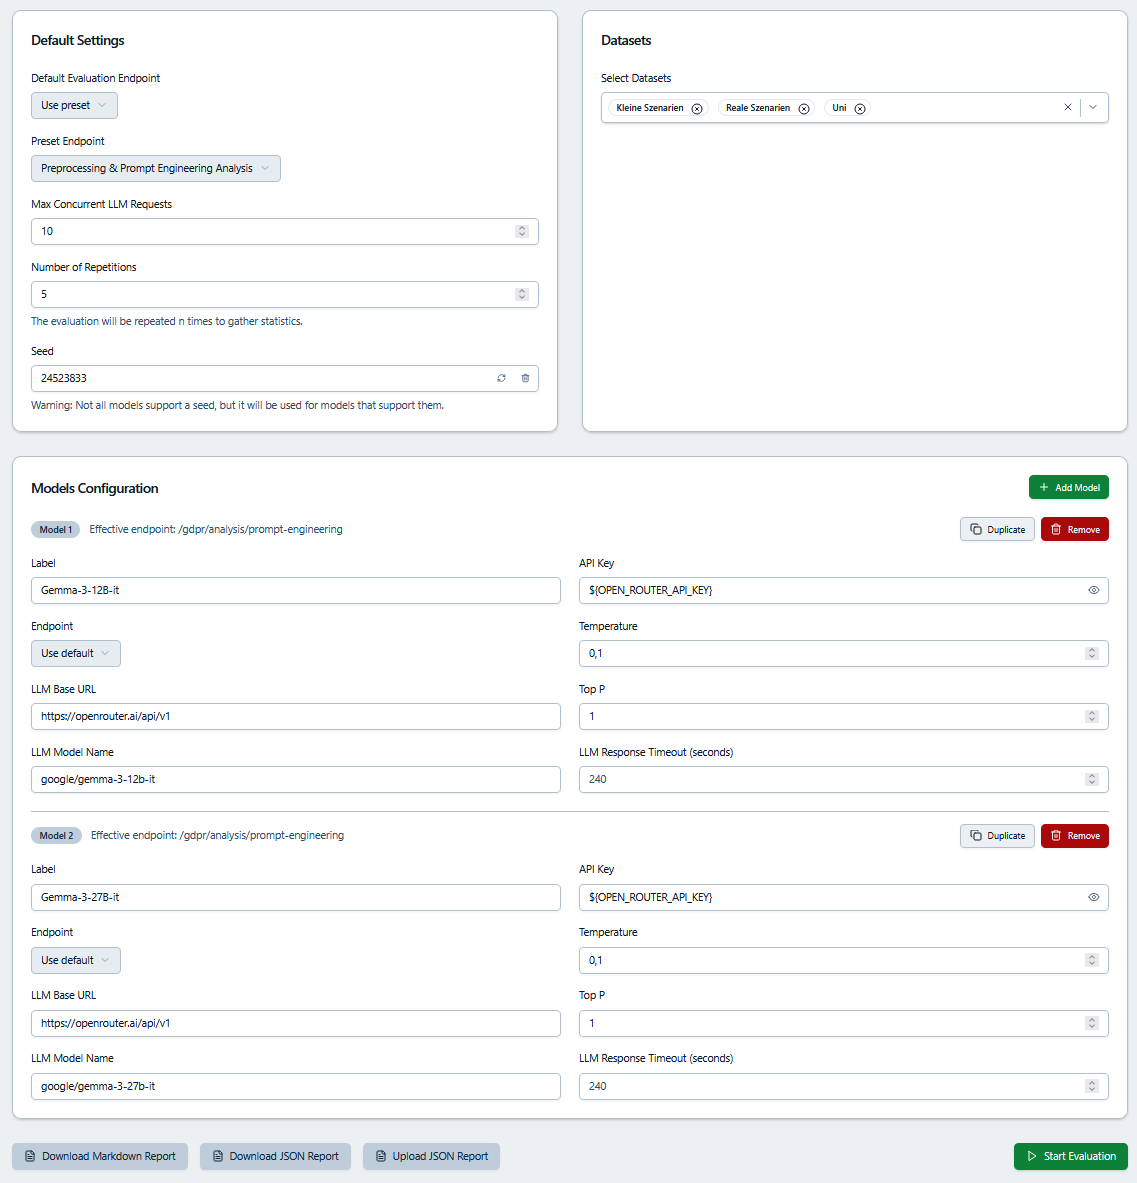
\includegraphics[width=\textwidth]{images/evaluation/evaluation-config_new}
    \caption{Formular zur Konfiguration einer Evaluation.}
    \label{fig:evaluation-config}
\end{figure}

\subsection*{Gesamtübersicht}

Nach dem Start der Evaluierung werden die Ergebnisse pro Modell inkrementell vom Backend übermittelt, im Frontend verarbeitet und in einer Gesamtübersicht wie in Abbildung \ref{fig:evaluation-overview} angezeigt. Dadurch können Teilergebnisse bereits untersucht werden, während die Evaluierung noch läuft. Die Gesamtübersicht bietet eine kompakte Zusammenfassung der Metadaten und der Kennzahlen aller Modelle über sämtliche Wiederholungen. So lassen sich die Modelle direkt miteinander vergleichen.

\begin{figure}[h]
    \centering
    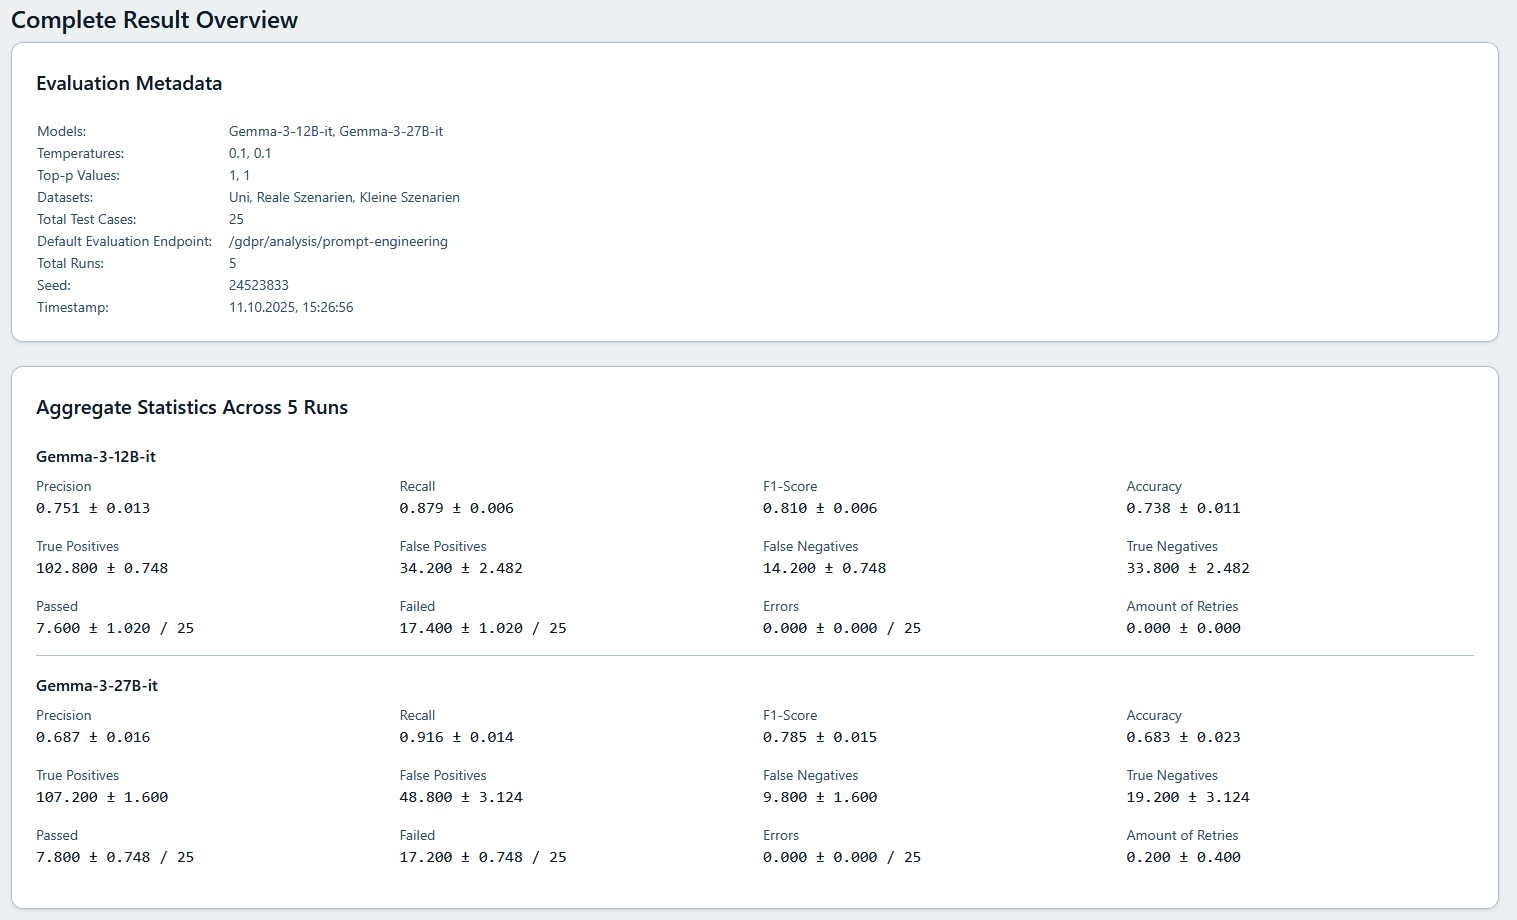
\includegraphics[width=\textwidth]{images/evaluation/evaluation-result-overview_new}
    \caption{Gesamtübersicht einer Evaluierung mit aggregierten Metriken über alle Wiederholungen.}
    \label{fig:evaluation-overview}
\end{figure}

\subsection*{Ergebnisse pro Wiederholung}

Die Übersicht der Ergebnisse pro Wiederholung ist in Abbildung \ref{fig:evaluation-by-run} dargestellt. Sie ermöglicht den Vergleich der Modelle innerhalb eines konkreten Laufs. So lassen sich die Kennzahlen einzelner Wiederholungen untersuchen und die Streuung der Ergebnisse zwischen den Läufen beurteilen. Zusätzlich werden die Anzahl der technisch fehlgeschlagenen Testfälle sowie die aufgetretenen Retries bei der Kommunikation mit dem \ac{LLM} angezeigt, um die Robustheit der Modelle bewerten zu können.

\begin{figure}[h]
    \centering
    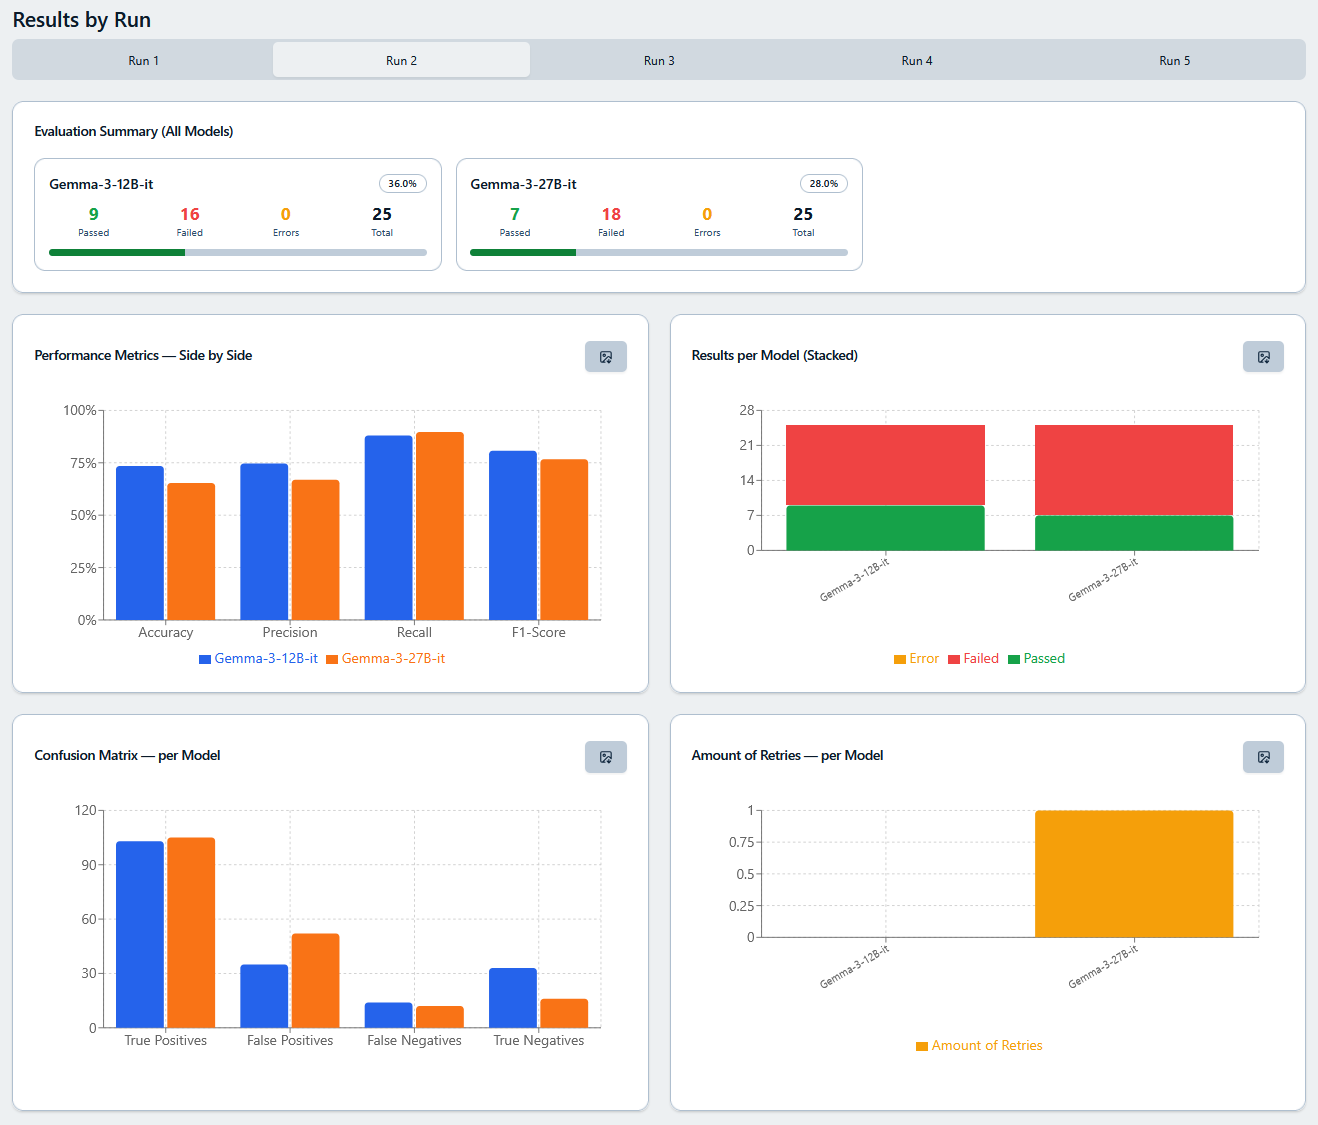
\includegraphics[width=\textwidth]{images/evaluation/evaluation-result-by-run_new}
    \caption{Ergebnisse pro Wiederholung mit exemplarischen Resultaten.}
    \label{fig:evaluation-by-run}
\end{figure}

\subsection*{Ergebnisse pro Modell}

Für eine vertiefte Analyse stellt das Frontend für jedes Modell eine Detailansicht bereit, die alle Kennzahlen über sämtliche Testfälle einer Wiederholung aggregiert. Abbildung \ref{fig:evaluation-by-model} zeigt diese Ansicht. Über Tabs kann zwischen den Modellen und Wiederholungen gewechselt werden, was einen schnellen Vergleich unterschiedlicher Modelle oder Läufe ermöglicht.

\begin{figure}[h]
    \centering
    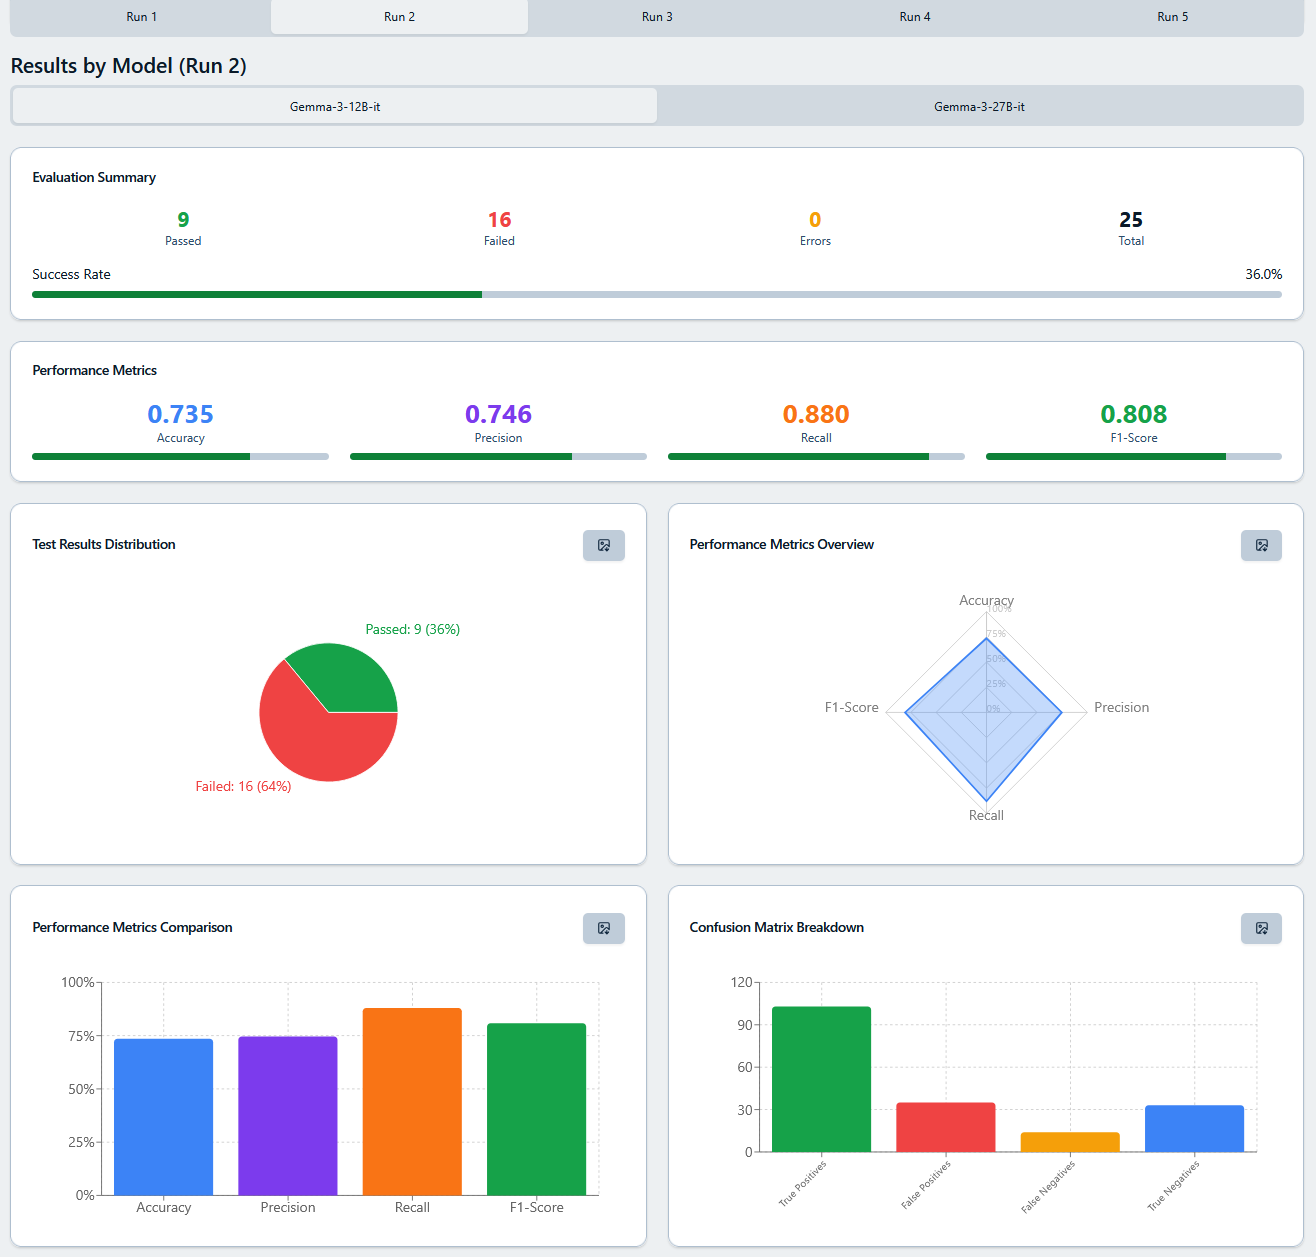
\includegraphics[width=\textwidth]{images/evaluation/evaluation-result-by-model_new}
    \caption{Modell-Detailansicht mit exemplarischen Ergebnissen.}
    \label{fig:evaluation-by-model}
\end{figure}

\subsection*{Ergebnisse pro Testfall}

Neben den aggregierten Ergebnissen pro Modell lassen sich auch die Resultate einzelner Testfälle je Modell untersuchen. Abbildung \ref{fig:evaluation-by-testcase} zeigt die Detailseite eines Testfalls. Sie enthält unter anderem den Status, die erwarteten gelabelten Aktivitäten und die vom Modell detektierten Aktivitäten. Zusätzlich visualisiert eine \ac{BPMN}-Darstellung den Prozess, und die Aktivitäten sind je nach korrekter oder inkorrekter Klassifizierung farblich markiert. Falls vorhanden, wird außerdem die vom  \ac{LLM} gelieferte Begründung pro Aktivität angezeigt.

\begin{figure}[h]
    \centering
    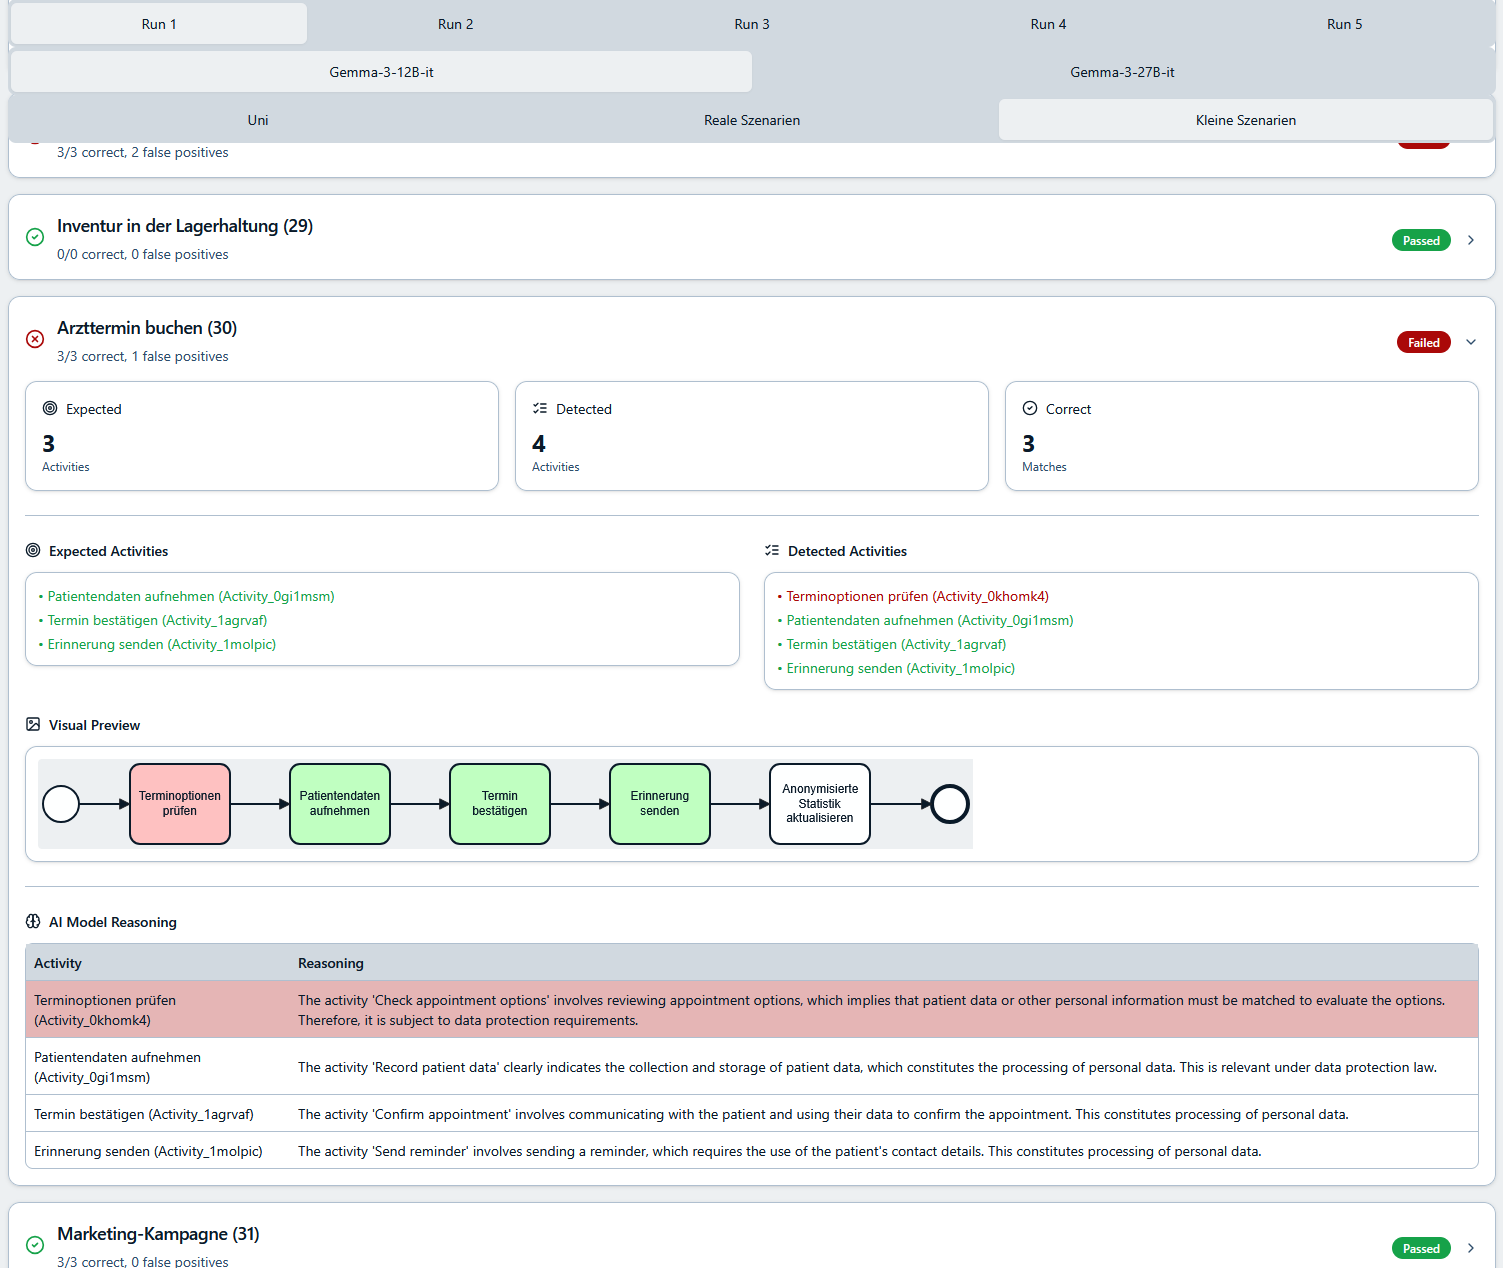
\includegraphics[width=\textwidth]{images/evaluation/evaluation-result-by-testcase_new}
    \caption{Detailseite eines Testfalls mit exemplarischen Ergebnissen.}
    \label{fig:evaluation-by-testcase}
\end{figure}.

Abweichungen werden dadurch unmittelbar sichtbar, und typische Fehlmuster wie systematische \ac{FP} bei bestimmten Aktivitätstypen lassen sich schnell erkennen. Testfälle, die aufgrund technischer Fehler nicht klassifiziert werden konnten, werden mit der entsprechenden Fehlermeldung aufgeführt. Über die Tabs am oberen Rand kann zwischen den Modellen, Wiederholungen und Testdatensätzen gewechselt werden, um verschiedene Perspektiven auf die Ergebnisse der Testfälle zu erhalten.
